\documentclass[border=10pt,margin=5pt,tikz,dvisvgm,rgb,utf8]{standalone}
\usepackage{ctex,xeCJK}  % 中文环境
\setCJKmainfont[BoldFont=Source Han Sans SC]{Source Han Serif SC}
\usepackage{calc,fontawesome,forest,smartdiagram,xcolor}
\usetikzlibrary{animations,arrows,automata,graphs,matrix,positioning,shadows,shapes}

\begin{document}
\renewcommand{\baselinestretch}{0.4}

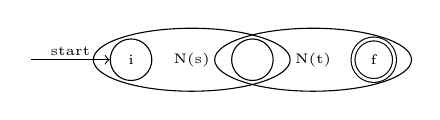
\begin{tikzpicture}
  \node[text width=-3em](Start){};
  \node[circle, draw=black, minimum width=15pt, minimum height=15pt, right=of Start](RI){\tiny i};
  \node[circle, draw=black, minimum width=15pt, minimum height=15pt, right=of RI](MID){\tiny \quad};
  \node[circle, double, double distance=1pt, draw=black, minimum width=15pt, minimum height=15pt, right=of MID](RF){\tiny f};

  \path[->]
  (Start) edge node[above=-2pt]{\tiny start} (RI)
  (RI) edge[draw=none] node{\tiny N(s)} (MID)
  (MID) edge[draw=none] node{\tiny N(t)} (RF);

  \draw ($(RI)!0.5!(MID)$) ellipse (1.25 and 0.4);
  \draw ($(MID)!0.5!(RF)$) ellipse (1.25 and 0.4);
\end{tikzpicture}

\end{document}
